\documentclass{article}

\title{Flat in-order binary trees}
\subtitle{An efficient algorithm for incremental merkle trees updates.}
\date{2023-08-13}
\modified{2023-11-26}

\keyword{cs}

\begin{document}
\section{sec-abstract}{Abstract}

This article is an in-depth guide to the flat in-order representation of binary trees.
We derive efficient operations to navigate these trees, such as finding the tree root and computing the parent and children for each node.
We then use this flat representation to implement a novel efficient data structure: extensible segment trees.

\section{sec-background}{Background}

Authenticated data structures are essential in distributed systems (e.g., version control systems and blockchains).
Binary \href{https://en.wikipedia.org/wiki/Merkle_tree}{Merkle trees} are among the most common approaches to authenticated data structures.

Building a Merkle tree from scratch for an arbitrary data structure is straightforward and can be mechanized\sidenote{sn-auth-ds-generically}{
See, for example, \href{https://www.cs.umd.edu/~mwh/papers/gpads.pdf}{Authenticated Data Structures, Generically} by Andrew Miller et al.
}.
A more interesting question is how to update existing Merkle trees incrementally to reflect changes in the underlying data structure.
For example, adding a new item to a sequence of \math{N} data blocks requires recomputing about \math{log\sub{2}(N)} hashes.

\begin{figure}[grayscale-diagram]
  \marginnote{mn-update-merkle-tree}{
    Adding a new item to a sequence of \math{N} data blocks requires recomputing about \math{log\sub{2}(N)} hashes in the Merkle tree.
    The diagram demonstrates the addition of the sixth node to a sequence of five data items.
    Hatched rectangles correspond to hash computations required to construct the new Merkle tree.
  }
  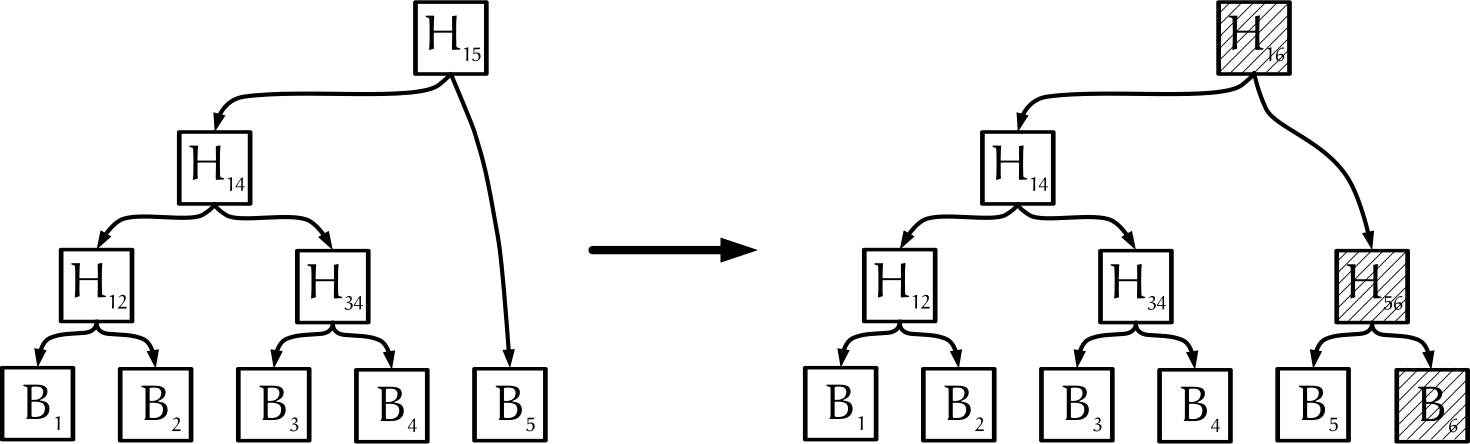
\includegraphics{/images/22-new-item.svg}
\end{figure}

Furthermore, storing Merkle trees for a linear sequence of data blocks explicitly (i.e., as explicit tree nodes with pointers) is wasteful.
Finding an \href{https://en.wikipedia.org/wiki/Implicit_data_structure}{implicit encoding} mapping the tree onto an array of \math{2N-1} hashes reduces storage space significantly.

The most common approach to packing a tree into an array used in binary heaps and \href{https://cp-algorithms.com/data_structures/segment_tree.html}{segment trees} is to place children of node at index \math{i} at positions \math{2i+1} and \math{2i+2}.
This approach works well for fixed-size arrays, but it's inefficient for growable arrays because adding a new data block might require \math{O(N)} data moves.

\begin{figure}[grayscale-diagram,medium-size]
  \marginnote{mn-binary-heap}{
    Representing a binary tree as an array using the \href{https://en.wikipedia.org/wiki/Binary_heap#Derivation_of_index_equations}{binary heap array indexing}.
    If a tree node maps to index \math{i}, then its left and right children map to indices \math{2i+1} and \math{2i+2} respectively.
  }
  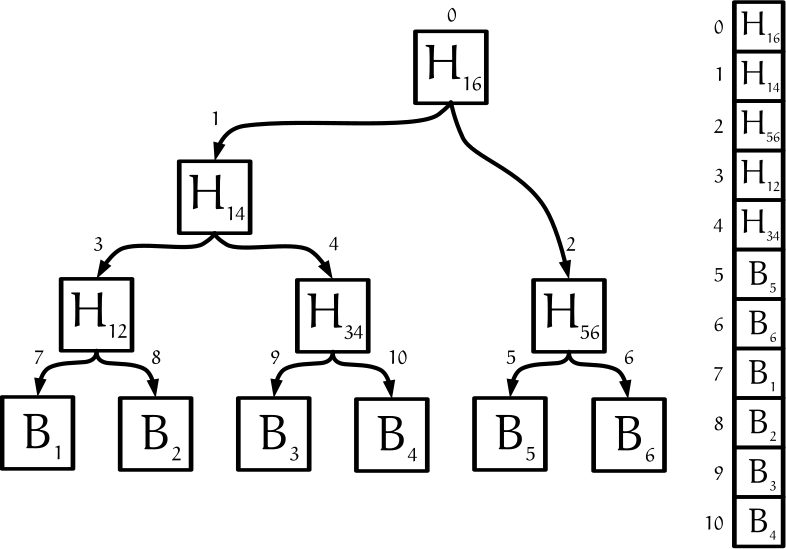
\includegraphics{/images/22-binary-heap.svg}
\end{figure}

The \href{https://www.datprotocol.com/}{DAT protocol} pioneered an alternative approach, \href{https://dat-ecosystem-archive.github.io/book/ch01-01-flat-tree.html}{flat in-order trees}.
This scheme interleaves interior node hashes and data hashes.
A tree with \math{N} data blocks requires \math{2N-1} slots, with \math{i}-th data block hash stored at index \math{2i}.
The interior hashes reside at odd indices between the data block hashes.
This scheme fixes the data node locations (slots with even indices contain leaf data nodes) and allows updating internal nodes efficiently.

\begin{figure}[grayscale-diagram,medium-size]
  \marginnote{mn-in-order-tree}{Representing a binary tree as an array using the flat in-order indexing.}
  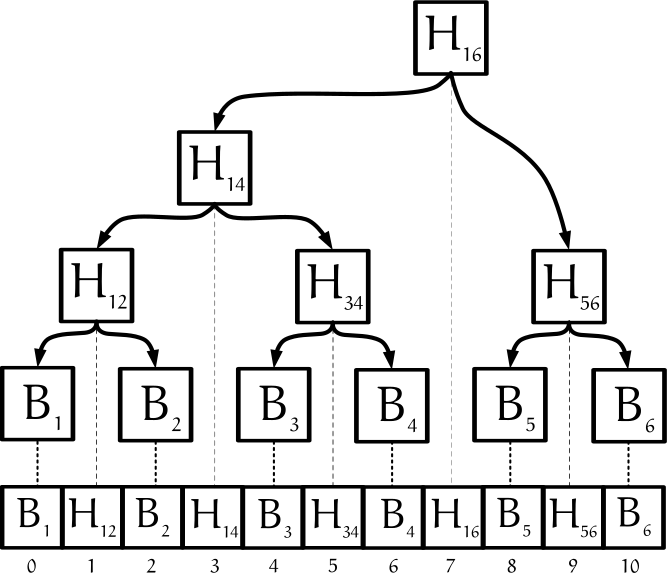
\includegraphics{/images/22-in-order-tree.svg}
\end{figure}

Unfortunately, the way DAT protocol defines trees is somewhat awkward: it treats the sequence as a forest of perfect binary trees, not a single binary tree.
Furthermore, the specification doesn't contain enough details on how to navigate the flat tree efficiently.

This article describes an intuitive model for flat in-order tree navigation and suggests efficient routines for computing the parent and children of any tree node.

\section{sec-nomenclature}{Nomenclature}

We will consider two types of trees.
First, we'll analyze the case of \emph{perfect binary trees} (\code{PBT}), i.e., binary trees in which all interior nodes have two children and all leaves have the same depth.
These trees correspond to sequences of \math{2\sup{K}} data blocks and contain \math{2\sup{K+1}-1} nodes.

Second, we'll generalize perfect trees to handle sequences of any \math{N} data blocks.
There is no established name for such trees, so we'll call them \emph{left-perfect binary trees} (\code{LPBT}).
A left-perfect tree with \math{N} leaves is either a perfect tree or a fork where the left child is a perfect tree containing at least \math{N/2} leaves, and the right child is a left-perfect tree containing the rest of the leaves.

\begin{figure}[grayscale-diagram,medium-size]
  \marginnote{mn-left-perfect-tree}{
    The left-perfect tree for a sequence of seven data blocks.
    Dotted rectangles mark perfect subtrees.
    The number of leaves in the perfect subtrees corresponds to powers of two in the binary representation of total leaf count.
  }
  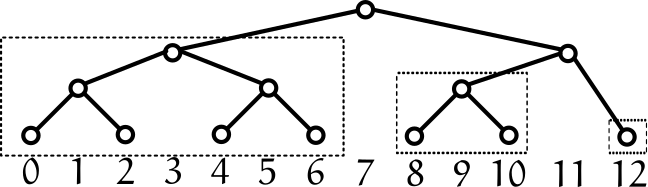
\includegraphics{/images/22-left-perfect-tree.svg}
\end{figure}

\section{sec-addressing}{Addressing tree nodes}

We'll first examine addressing nodes within a flat in-order perfect binary tree and then extend the approach to left-perfect binary trees.

\sc{theorem}: in a flat in-order perfect binary tree of depth \math{D}, node's index \math{i} has the following structure:
\begin{itemize}
    \item
    The longest run of least-significant set bits in \math{i}'s binary representation indicates the depth of subtrees rooted at \math{i}.
    If \math{i}'s binary representation has the last \math{K} bits set, \math{i}'s children are subtrees of depth \math{K}.
    \item
    The bits before the last zero signify the path to node \math{i} starting from the tree root.
    Zeros indicate left turns; ones indicate right turns.
\end{itemize}

\begin{figure}[grayscale-diagram,medium-size]
  \marginnote{mn-addressing-scheme}{
    The addressing scheme for nodes in the flat in-order representation of perfect binary trees.
  }
  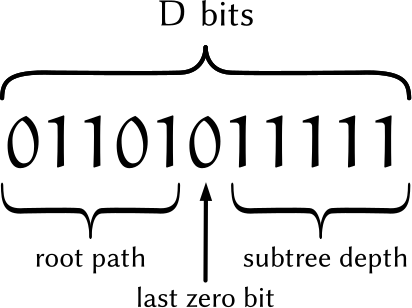
\includegraphics{/images/22-addressing-scheme.svg}
\end{figure}

\sc{proof}: by induction on the tree depth \math{D}.

Base case: the theorem is vacuously true for trees of depth one (a single node with index zero).
The case of a tree of depth two is more instructive:

\begin{figure}[grayscale-diagram]
  \marginnote{mn-addressing-scheme}{
    An example of the in-order addressing scheme for a tree of depth two.
  }
  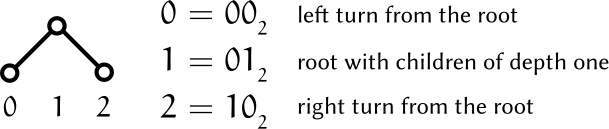
\includegraphics{/images/22-depth-two-example.svg}
\end{figure}

Induction step: let's assume that the theorem holds for trees of depth \math{D} and consider a tree of depth \math{D+1}.

\begin{figure}[grayscale-diagram]
  \marginnote{mn-visual-proof}{
    The induction step of the flat in-order tree addressing theorem.
  }
  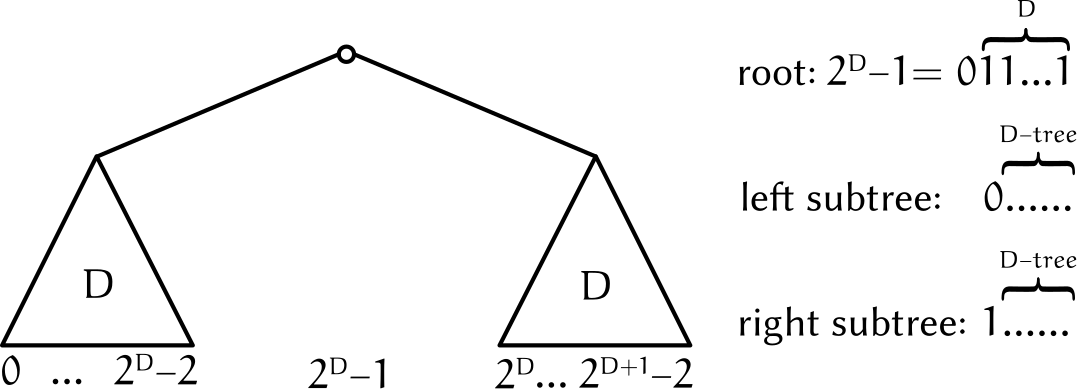
\includegraphics{/images/22-visual-proof.svg}
\end{figure}

The root of a \math{D+1}-tree resides at index \math{2\sup{D}-1}, so its binary representation is \math{011\ldots 1}, with precisely \math{D} least-significant bits set.
The binary representation of indices in the left subtree starts with zero, followed by a \math{D}-tree address.
The binary representation of indices in the right subtree begins with one, followed by a \math{D}-tree address.
Hence, the addressing scheme preserves as we increase the tree depth from \math{D} to \math{D+1}.
\qed

\section{sec-fbt}{Traversing perfect binary trees}

We'll need two primitive bit-twiddling operations for the tree navigation: locating the last zero bit of a number and rounding a number up to a power of two\sidenote{sn-examples-c}{
  All code in this article is in the \href{https://en.wikipedia.org/wiki/C_(programming_language)}{C programming language} and complies with the \href{https://en.wikipedia.org/wiki/C11_(C_standard_revision)}{C11 standard}.
}.

\begin{code}[c]
#include <assert.h>
#include <stdint.h>

\emph{// Isolates the last set bit of number N.}
uint64_t LastSetBit(const uint64_t n) {
    return n - ((n - 1) & n);
}

\emph{// Isolates the last unset bit of number N.}
uint64_t LastZeroBit(const uint64_t n) {
    return LastSetBit(n + 1);
}

\emph{// Rounds the argument up to the next highest power of two.}
uint64_t RoundUpPowerOf2(uint64_t n) {
    // See \href{https://graphics.stanford.edu/~seander/bithacks.html#RoundUpPowerOf2}{Bit Twiddling Hacks}.
    n--;
    n |= n >> 1;
    n |= n >> 2;
    n |= n >> 4;
    n |= n >> 8;
    n |= n >> 16;
    n |= n >> 32;
    n++;
    return n;
}
\end{code}

We are now ready to define the tree navigation functions.
The addressing scheme proof suggests the function for locating the tree root: we divide the tree size by two.

\begin{code}[c]
\emph{// Computes the root of the perfect binary tree of the given SIZE.}
uint64_t PBT_Root(const uint64_t size) {
    assert(size == 1 || RoundUpPowerOf2(size) == size + 1);
    return size >> 1;
}
\end{code}

Next, let's consider locating the parent of node \math{i}.
According to the scheme, we must find the last zero in the binary representation of \math{i}, set it to one, and set the next most significant bit to zero.

\begin{figure}[grayscale-diagram,medium-size]
  \marginnote{mn-fbt-parent}{
    The relation between binary representations of node \math{i} and its parent \math{p} in a flat in-order perfect binary tree.
    If bit \math{b\sub{k}} is zero, then \math{i} is the left child. Otherwise, \math{i} is the right child.
  }
  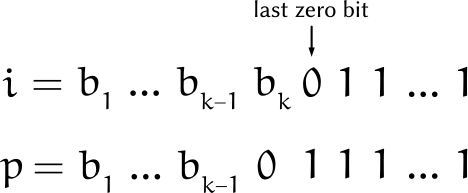
\includegraphics{/images/22-fbt-parent.svg}
\end{figure}

\begin{code}[c]
\emph{// Computes the parent of node I in a perfect binary tree.}
uint64_t PBT_Parent(const uint64_t i) {
    return (LastZeroBit(i) | i) & ~(LastZeroBit(i) << 1);
}
\end{code}

Finally, the parent computation suggests procedures for locating the children.
We must find the last zero bit \math{k} in the node's binary representation.
For the left child, we must set bit \math{k-1} to zero.
For the right child, we also need to set bit \math{k} to one.

\begin{code}[c]
\emph{// Computes the left child of node P in a perfect binary tree.}
\emph{// Requires: P is not a leaf.}
uint64_t PBT_LeftChild(const uint64_t p) {
    assert(p & 1);
    return p & ~(LastZeroBit(p) >> 1);
}

\emph{// Computes the right child of node P in a perfect binary tree.}
\emph{// Requires: P is not a leaf.}
uint64_t PBT_RightChild(const uint64_t p) {
    assert(p & 1);
    return (p | LastZeroBit(p)) & ~(LastZeroBit(p) >> 1);
}
\end{code}

Next, we'll generalize these functions to handle left-perfect binary trees.

\section{sec-lpbt}{Traversing left-perfect binary trees}

The left subtree of a left-perfect binary tree is a perfect binary tree by definition.
Hence the formula for the left child we developed for perfect binary trees works as-is.

\begin{code}[c]
\emph{// Computes the left child in a flat in-order left-perfect binary tree.}
uint64_t LPBT_LeftChild(const uint64_t i) { return PBT_LeftChild(i); }
\end{code}

We need three more operations to efficiently navigate a left-perfect binary tree: finding the tree root and computing the node's parent and right child.
Left-perfect binary tree structure changes with the node count, so the latter two functions will depend on the node index and the tree node count.

\begin{figure}[grayscale-diagram]
  \marginnote{mn-cbt-structure}{
    In a left-perfect binary tree, the tree structure changes as the tree grows.
    The parent of node 4 in a five-node tree is node 3, but it becomes node 5 when we add one more leaf.
  }
  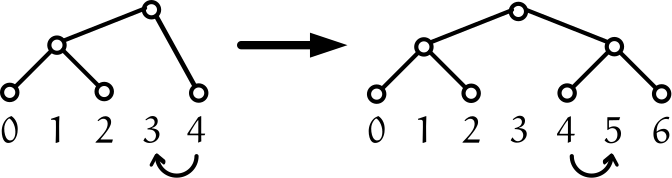
\includegraphics{/images/22-cbt-structure-change.svg}
\end{figure}

In a left-perfect binary tree, the tree root is the same node that the smallest perfect binary tree with at least the same number of nodes would have.
Thus, given the number of tree nodes, we compute the root of the smallest perfect tree containing the input tree.

\begin{code}[c]
\emph{// Computes the root of a left-perfect binary tree of the given SIZE.}
uint64_t LPBT_Root(const uint64_t size) {
    return PBT_Root(RoundUpPowerOf2(size + 1) - 1);
}
\end{code}

Another way to view left-perfect binary trees is to imagine them as perfect binary trees with some trailing nodes removed.
The remaining nodes are reattached to the closest existing parent to keep the tree complete.
This observation gives us a simple way to compute the node's parent:
We apply the \code{PBT_Parent} function until the computed node falls within the tree bounds.

\begin{figure}[grayscale-diagram]
  \marginnote{mn-missing-nodes}{
    We can see a left-perfect binary tree as a perfect binary tree with some of the trailing nodes in the right subtree removed.
    Note that all of the missing nodes are outside of the tree.
    Following node's ``virtual'' parents until we hit a ``real'' node gives us the node's true parent.
  }
  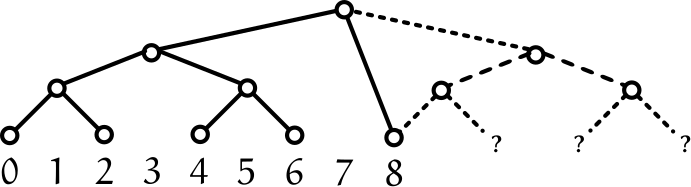
\includegraphics{/images/22-missing-nodes.svg}
\end{figure}

\begin{code}[c]
\emph{// Computes the parent of node I in a left-perfect binary tree of the given SIZE.}
uint64_t LPBT_Parent_Iterative(uint64_t i, const uint64_t size) {
    do { i = PBT_Parent(i); } while (i >= size);
    reutrn i;
}
\end{code}

There is also a non-iterative way to find the parent in a left-perfect tree.
Notice that the \code{PBT_Parent} function can return a value outside the array only if the input node is either the root node or a right child\sidenote{sn-parent-right-proof}{
Proof: if the node is a left child, then it's a root of a perfect binary tree (by definition of left-perfect trees), and its parent resides to its right within the array bounds (by construction of in-order trees).
}.
Furthermore, if node \code{i} is a right child, its parent is always the node preceding \code{i}-th most-left leaf. 
Thus, we can attempt to compute the parent using \code{PBT_Parent} first and adjust the result if it falls out of bounds.

\begin{code}[c]
\emph{// Computes the leftmost leaf of node I in a perfect binary tree.}
uint64_t PBT_LeftmostLeaf(const uint64_t i) {
    return i & (i + 1);
}

\emph{// Computes the parent of node I in a left-perfect binary tree of the given SIZE.}
uint64_t LPBT_Parent(const uint64_t i, const uint64_t size) {
    assert(i != LPBT_Root(size));
    const uint64_t p = PBT_Parent(i);
    return (p < size) ? p : PBT_LeftmostLeaf(i) - 1;
}
\end{code}

Our observations give us two algorithms for computing the right child.
Notice that the \code{PBT_RightChild} function gives correct results if the output value falls within the tree bounds.
If the outcome falls outside the tree bounds, the recursive definition of left-perfect trees implies that the right child must be the root of the right subtree.

\begin{code}[c]
\emph{// Computes the right child of node I in a left-perfect binary tree of the given SIZE.}
uint64_t LPBT_RightChild(const uint64_t i, const uint64_t size) {
    assert(n & 1);
    const uint64_t r = PBT_RightChild(i);
    return (r < size) ? r : i + 1 + LPBT_Root(size - i - 1);
}
\end{code}

Alternatively, if \code{PBT_RightChild}'s result falls outside of the tree, we can follow the left links in the ``virtual'' perfect tree until we hit the tree bounds again.

\begin{code}[c]
\emph{// Computes the right child of node I in a left-perfect binary tree of the given SIZE.}
uint64_t LPBT_RightChild_Iterative(const uint64_t i, const uint64_t size) {
    assert(n & 1);
    uint64_t r;
    for (r = PBT_RightChild(n); r < size; r = PBT_LeftChild(r));
    return r;
}
\end{code}

We now have enough tools to navigate any left-perfect binary tree efficiently.

\section{sec-extensible-segment-trees}{Extensible segment trees}

Merkle trees are a special case of \href{https://cp-algorithms.com/data_structures/segment_tree.html}{segment trees}.
Traditional representations of segment trees allow efficient updates, but they don't support appending new items to the sequence.
Flat in-order representation for segment trees opens a path to an efficient append operation.

This section presents an implementation of segment trees designed for answering range sum queries.
The same approach will work for any problem where node elements and the aggregation operation form a \href{https://en.wikipedia.org/wiki/Semigroup}{semigroup}.

We'll need a new operation to support efficient range queries: finding the \href{https://en.wikipedia.org/wiki/Lowest_common_ancestor}{lowest common ancestor} (LCA) of two leaves in a left-perfect binary tree.
The \href{#sec-addressing}{tree addressing scheme} suggests a simple way to compute LCA for leaves because their paths from the root node are aligned.
We must find the most significant bit where the leaves differ, set this bit to zero, and set all lower bits.

\begin{code}[c]
\emph{// Extracts the most significant bit from number N.}
uint64_t MostSignificantBit(uint64_t n) {
    uint64_t x = n;
    x |= (x >> 1);
    x |= (x >> 2);
    x |= (x >> 4);
    x |= (x >> 8);
    x |= (x >> 16);
    x |= (x >> 32);
    return x - (x >> 1);
}

\emph{// Computes the lowest common ancestor of leaves X and Y in a left-perfect}
\emph{// binary tree.}
uint64_t LPBT_LeavesLCA(const uint64_t x, const uint64_t y) {
    assert(!(x & 1));
    assert(!(y & 1));

    if (x == y) return x;
    const uint64_t d = MostSignificantBit(x ^ y);
    return (x & ~d) | (d - 1);
}
\end{code}

We can now proceed with the segment tree implementation.
Let's define the data structures representing the tree.

\begin{code}[c]
\emph{// The type of values stored in the tree nodes.}
typedef int64_t value_t;

\emph{// The maximum number of nodes in the tree.}
const size_t MAX_NODES = 10001;

\emph{// The current number of nodes in the tree.}
\emph{// Invariant: G_NumNodes <= MAX_NODES}
\emph{// Invariant: G_NumNodes == 0 || G_NumNodes \% 2 == 1}
size_t G_NumNodes;

\emph{// The flat in-order representation of the tree.}
\emph{// Even elements correspond to the sequence items.}
value_t G_Nodes[MAX_NODES];
\end{code}

We highlight that the trees work with any semigroup by extracting the combining operator into a separate function.

\begin{code}[c]
value_t Combine(const value_t x, const value_t y) {
    return x + y;
}
\end{code}

We then define procedure \code{ST_Set} updating the sequence.
It sets the corresponding leaf value and traverses the tree upwards, recomputing the parent node values.

\begin{code}[c]
\emph{// Updates the sequence to contain the given ITEM at the specified POSITION.}
void ST_Set(const size_t position, const value_t item) {
    assert(G_NumNodes > 0);
    assert(position <= G_NumNodes / 2);

    size_t i = position * 2;
    G_Nodes[i] = item;

    if (G_NumNodes == 1) return;

    size_t root = LPBT_Root(G_NumNodes);
    do {
        i = LPBT_Parent(i, G_NumNodes);
        G_Nodes[i] = Combine(
            G_Nodes[LPBT_LeftChild(i)],
            G_Nodes[LPBT_RightChild(i, G_NumNodes)]
        );
    } while (i != root);
}
\end{code}

The \code{ST_Append} procedure adds an item to the sequence and updates the tree accordingly.
The empty sequence is a special case because there are no interior nodes to update.
In the case of non-empty sequences, the procedure adds a new interior node and a leaf and delegates the rest to the previously defined \code{ST_Set} procedure.

\begin{code}[c]
\emph{// Appends the given ITEM to the sequence.}
void ST_Append(const value_t item) {
    assert(G_NumNodes + 2 <= MAX_NODES);

    if (G_NumNodes == 0) {
        G_Nodes[G_NumNodes++] = item;
    } else {
        G_NumNodes += 2;
        ST_Set(G_NumNodes / 2, item);
    }
}
\end{code}

The \code{ST_Sum} function computing the sum of sequence items in the specified range is the most involved part of the implementation.
It relies on the \code{LPBT_LeavesLCA} function to compute the LCA of the two leaves corresponding to the requested bounds.
It then traverses the tree from the left bound to the LCA node, summing all unaccounted \emph{right} subtrees on the way up.
It does the same for the right bound, summing all unaccounted \emph{left} subtrees on the path.

\begin{figure}[grayscale-diagram]
  \marginnote{mn-lca-sum}{
    Computing the sum of items in the range from sequence item \math{l = 1} (node index \math{i = 2}) to item \math{r = 5} (node index \math{j = 10}) in a flat in-order tree using traversal to the lowest common ancestor.
    Dotted rectangles mark subtrees to be accumulated.
  }
  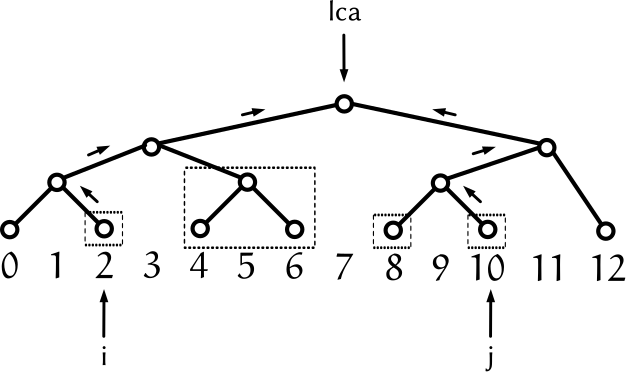
\includegraphics{/images/22-lca-sum.svg}
\end{figure}

\begin{code}[c]
\emph{// Computes the sum of the sequence items in the index interval \[l, r\].}
value_t ST_Sum(const size_t l, const size_t r) {
    assert(r * 2 < G_NumNodes);
    assert(l <= r);

    uint64_t i = l * 2;
    uint64_t j = r * 2;

    if (i == j) return G_Nodes[i];

    const uint64_t lca = LPBT_LeavesLCA(i, j);
    value_t acc = Combine(G_Nodes[i], G_Nodes[j]);

    \emph{// Traverse the tree upwards from the left bound and sum up all}
    \emph{// the right subtrees on the way.}
    while (1) {
        const uint64_t p = LPBT_Parent(i, G_NumNodes);
        if (p == lca) break;

        const uint64_t rc = LPBT_RightChild(p, G_NumNodes);
        if (rc != i) acc = Combine(acc, G_Nodes[rc]);
        i = p;
    }
    \emph{// Traverse the tree upwards from the right bound and sum up all}
    \emph{// the left subtrees on the way.}
    while (1) {
        const uint64_t p = LPBT_Parent(j, G_NumNodes);
        if (p == lca) break;

        const uint64_t lc = LPBT_LeftChild(p);
        if (lc != j) acc = Combine(acc, G_Nodes[lc]);
        j = p;
    }
    return acc;
}
\end{code}

The \code{ST_Append}, \code{ST_Set}, and \code{ST_Sum} procedures provide a working implementation of extensible segment trees.

\end{document}
